\section{Hardware development}
\label{sec:hardware}
This section describes the development of the hardware of the stepper motor controller.
Firstly, the critical components are selected and preliminary design is done based on the requirements stated in the Section ~\ref{sec:requirements}.
Secondly, both of the hardware revisions and their design are described.

\subsection{Hardware Design Choices}
\label{subsec:hardware_design_choices}
In this section, we describe the choices made in the beginning of the design process, ones that are vital to the functionality of the whole system.
The design choices are based on the requirements~\ref{sec:requirements}, the related work described in the Chapter~\ref{ch:related_work} and our prior experience.

\subsubsection{MCU}
\label{subsubsec:mcu}
One of the critical components of the stepper controller is the MCU.
The MCU needs to accommodate for the outer communication interfaces as well as the internal ones.
That means that as for the outer communication interfaces, it needs to have peripherals for CAN bus, I\textsuperscript{2}C and USB, as stated in the requirement \textbf{C-03}.
The internal communication interfaces are revision dependent, however the stepper controllers generally require, GPIOs, PWM outputs, serial interfaces and for the possible future encoder support it should require incremental encoder interfaces and SPIs for SSI bitbanging (as stated in requirement \textbf{FR-08}).
As was described in the Chapter on Related work~\ref{ch:related_work}, we decided to make the move from Cortex-M0 and Cortex-M0+ based ARM MCUs to more powerful Cortex-M4 MCUs.
The biggest advantage of these cores is that they fully support atomic instructions, improving memory safety in ISRs, and also that they have FPU (Floating Point Unit).

Given the past experience with STM32 family of ARM microcontrollers, we decided to select the STM32F4 product line, more specifically with the STM32F405RGT6 which features one megabyte of flash and 192 kilobytes of RAM and can be run with the 168 MHz clock\cite{stmicro_stm32f405rg_nodate}.
The block diagram of the MCU with the core features and peripherals can be seen in the Figure~\ref{fig:stm32f405_block_diagram}.

\begin{figure}[H]
    \centering
    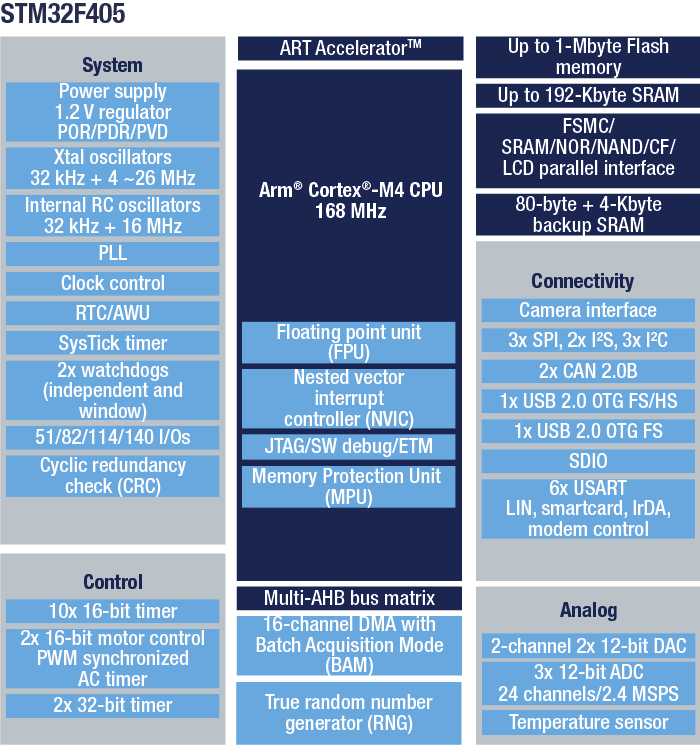
\includegraphics[width=0.7\textwidth]{obrazky/stm32f405_block_diagram}
    \caption{The block diagram of the STM32F405RG MCU~\cite{stmicro_enbd_stm32f405_1mbjpg_nodate}.}
    \label{fig:stm32f405_block_diagram}
\end{figure}

This MCU conforms to all of the requirement and has enough peripherals to support future development.

% FIXME reference Stepper Driver ic comparison
\subsubsection{Stepper driver}
\label{subsubsec:stepper_driver}
As per the requirements \textbf{C-01} and \textbf{C-02}, the stepper driver shall be able to drive stepper motors with current of up to 2A and feature silent operation.
We decided to use the stepper motor driver ICs developed by Trinamic.
These drivers are nowadays being used for motion control of 3D printers~\cite{prusa_trinamic} and allow for silent operation with their StealthChop technology.
When selecting the driver ICs there were different priorities in mind - first the package should be solderable by hand, secondly with the first revision of the SM4 stepper motor controller we aimed for the ability to power the drivers via a 10-cell Li-Ion power pack, which required maximal input voltage of more than 42 Volts.
The first hardware revision features the TMC2100-TA driver IC, whose main features are shown in the Table~\ref{tab:tmc2100_param}.

\begin{table}[H]
    \centering
    \begin{tabular}{ |p{5cm}|p{7cm}| }
        \hline
        Parameter & Value \\
        \hline
        \hline
        Motor supply voltage & 5-46 V \\
        \hline
        Microsteps & up to 256 \\
        \hline
        Control interface & Step/Dir \\
        \hline
        Configuration interface & GPIO \\
        \hline
        Phase current (RMS) & 1.4 A \\
        \hline
        Advanced stepper control technologies & MicroPlyer, SpreadCycle, StealthChop \\
        \hline
        Package & eTQFP48 \\
        \hline
    \end{tabular}
    \caption{Main parameters of the Trinamic TMC2100-TA driver IC~\cite{trinamic_tmc2100-datasheet_2018}.}
    \label{tab:tmc2100_param}
\end{table}


With the second hardware revision, the priorities have shifted and higher phase current was required (\textbf{C-01}) even at the expense of the supply voltage.
The second hardware revision features the TMC2226-SA driver IC, whose properties are shown in the Table~\ref{tab:tmc2226_param}.

\begin{table}[H]
    \centering
    \begin{tabular}{ |p{5cm}|p{7cm}| }
        \hline
        Parameter & Value \\
        \hline
        \hline
        Motor supply voltage & 4.75-29 V \\
        \hline
        Microsteps & up to 256 \\
        \hline
        Control interface & Step/Dir or UART \\
        \hline
        Configuration interface & UART \\
        \hline
        Phase current (RMS) & 2.0 A \\
        \hline
        Advanced stepper control technologies & MicroPlyer, CoolStep, SpreadCycle, StealthChop2, StallGuard4 \\
        \hline
        Package & HTSSOP28 \\
        \hline
    \end{tabular}
    \caption{Main parameters of the Trinamic TMC2226-SA driver IC~\cite{trinamic_tmc2226_2020}.}
    \label{tab:tmc2226_param}
\end{table}


% TODO read and refactor
\subsubsection{SM4 stepper driver power design}
\label{subsubsec:power_design}
The power design of the SM4 stepper motor controller is fairly simple.
According to the requirements, the only requirement for it is to provide basic electrical safety features, such as fuses and reverse voltage protection \textbf{FR-07}.
The controller features two power rails - one for the power electronics, that can utilize quite high voltages and one 5~V for the MCU and the peripheral circuits.
With the first revision, we were considering using a single power-rail with all voltages derived from the power electronics one.
This was however dismissed as a buck converter from quite a high voltage would be required and designing a buck converter is out of the scope of this project and also the motor controller was never meant to be use as a standalone device, meaning that another device could provide the power for the 5~V rail.
The buck converter would also pose EMI (ElectroMagnetic Interference) problems and would increase the price of the motor controller.

As for the power electronics, only input voltage filtering using capacitors was utilized.
The main reasoning being that this should be fused on the side of the power source and that reverse-voltage protection would require quite large components.

The situation is different with the 5~V power rail for peripherals and the MCU.
This power rail utilizes 500~mA PTC fuse, reverse-voltage protection implemented using P-channel MOSFET and a low-pass filter comprising of a ferrite bead and a capacitor.
This power rail is connected to the connectors with CAN bus and I\textsuperscript{2}C.
The output of the filtered power rail is merged with a 5~V power coming from the USB-C connector (which is also fused using a 500~mA PTC fuse) using Schottky diodes.
For powering the MCU with 3.3~V, the 5~V is regulated with an LDO (Low-Dropout) regulator.
The whole power rail can be seen in the schematic in the Figure~\ref{fig:power}.

In the future revisions, the input protection circuits may be replaced by an eFuse\cite{efuse_great_scott}\cite{efuse}, an IC integrating the input power protection circuits such as overvoltage protection, undervoltage protection, overcurrent protection and reverse-voltage protection.

\begin{figure}[H]
    \centering
    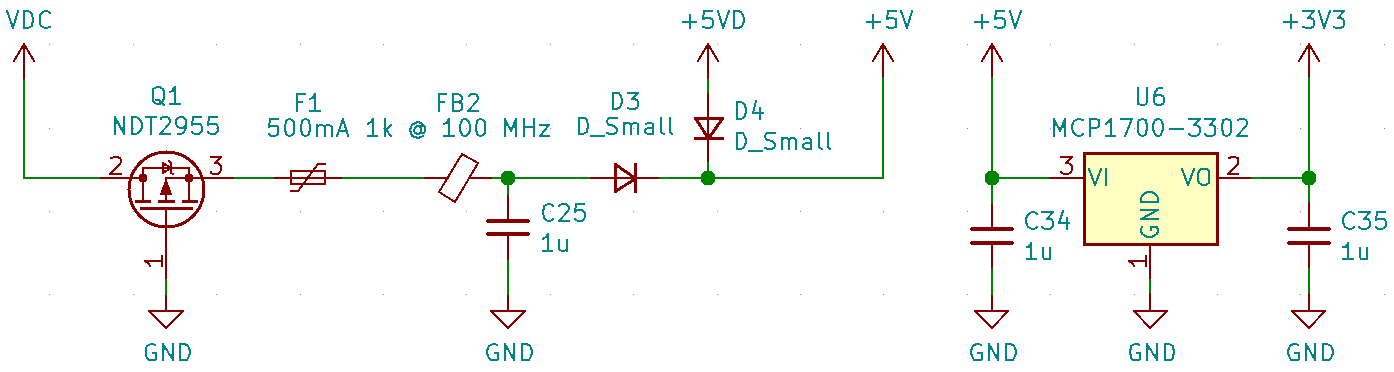
\includegraphics[width=0.9\textwidth]{obrazky/power}
    \caption{The 5~V power rail for powering the MCU and peripherals.}
    \label{fig:power}
\end{figure}

\subsubsection{PCB Design}
\label{subsubsec:pcb_design}
In order for this project to serve as a testbed for new manufacturing technologies, the PCB (Printed Circuit Board) was designed as 4-layer.
The ability to design the board as a 4-layer one was enabled by the 4-layer PCB manufacturing price decrease by China-based PCB manufacturing companies.
Big advantage of designing the PCB as 4-layer one was speedup of hardware development - the 4-layer stackup can be utilized so that there is no need to route power to the ICs.
In our case we chose the inner layers to be filled with copper planes - one connected to GND and the other one connected to +3.3~V.
This way whenever a connection to +3.3V or GND was required, simply connecting the pad to new via close-by was sufficient.
Apart from being used for power distribution, the large copper planes allow for better PCB cooling and also for some minor signal connections in cases routing using the outer layers would prove difficult.
The used stackup can be seen in the Figure~\ref{fig:stackup}.

\begin{figure}[H]
    \centering
    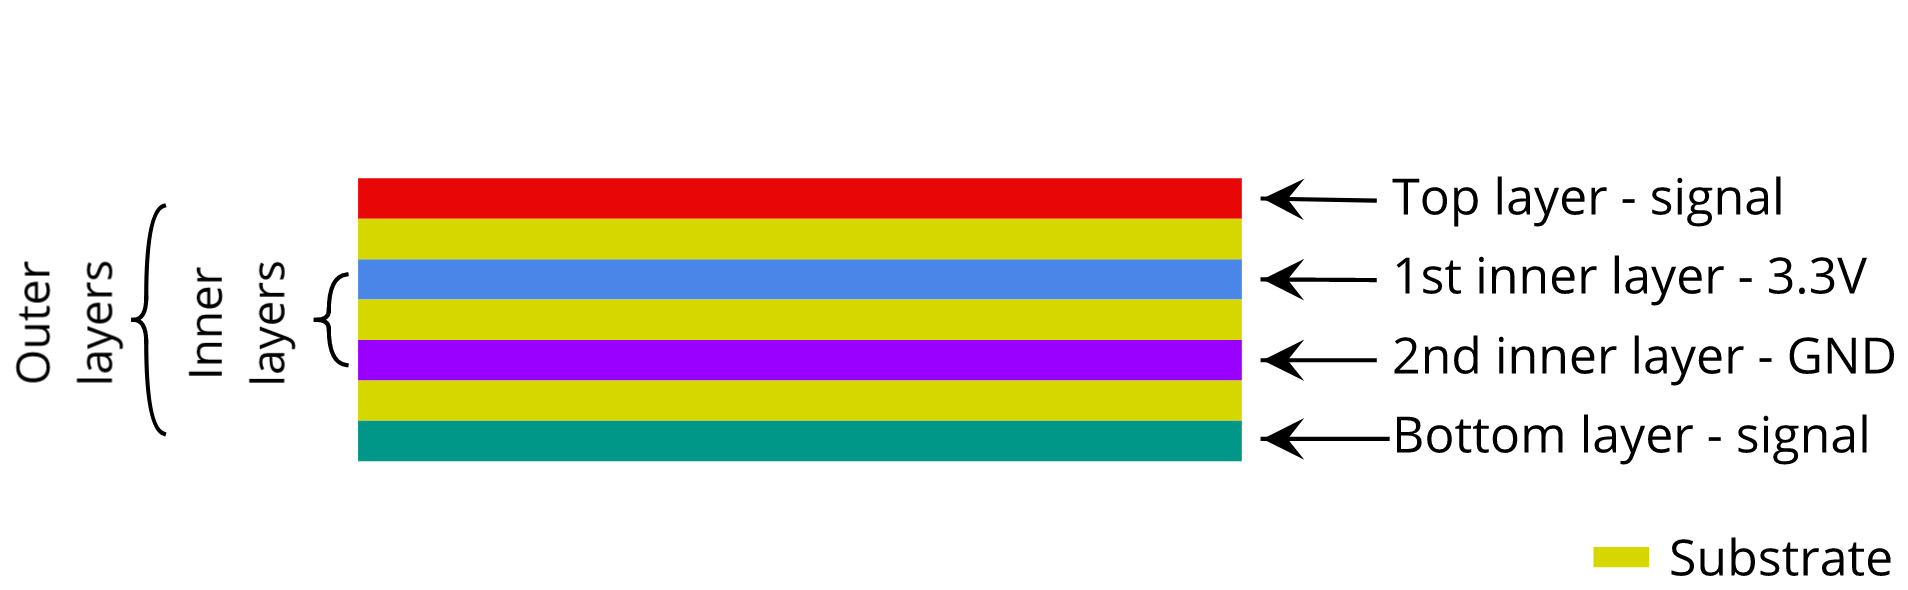
\includegraphics[width=0.9\textwidth]{obrazky/stackup}
    \caption{The 4-layer PCB stackup.}
    \label{fig:stackup}
\end{figure}

Another way to test manufacturing capabilities was utilizing the automated assembly service provided by the China-based PCB manufacturers.
This not-only saved a lot of time with manual assembly, but also enabled us to use smaller components than before - the imperial size 0402.

As for testing out EDA (Electronic Design Aid) software, the KiCAD EDA was used instead of the well-known Eagle.
The KiCAD EDA has improved dramatically in the past years (version 5 and soon to be released version 6), making it great competitor to conventional EDA suites.
The big advantage of KiCAD is a large footprint and symbol library, which often contains even the 3D models and KiCAD itself is able to seamlessly integrate them and render a 3D view of the designed PCB.

